\section{技能编译}
\label{sec:compiler}

当用户首次安装技能时，\sys 会在技能尚未运行前，针对目标端（模型、代理框架、主机环境）编译该技能。
编译器读取原始技能文本，识别目标端，
并经过三个顺序阶段生成一个或多个优化后的\emph{技能变体}。
每个阶段弥合一种不同的缺口，即技能预期与目标端实际提供的内容之间的差异。

\subsection{基于能力的编译}
\label{sec:compiler:cap}

第一个阶段处理模型与代理框架的错配。
由于目标端差异很大（\S\ref{sec:insight:challenges}），
编译器不能内置针对每个目标端的优化逻辑。
为此，\sys 引入\emph{原语能力}，
作为一种抽象词汇，用于表达技能需要什么，以及目标端能够提供什么。
编译器离线使用针对这些能力的微基准对每个目标端进行画像，
将画像结果与技能的能力需求比较，
并根据两者之间的缺口选择优化策略。

\subsubsection{原语能力}

正如 JVM 字节码定义 Java 程序要求其运行时提供的基本操作，
原语能力定义技能要求其目标端提供的基本能力。
原语能力是一个不可再分的单元，用来描述完成技能所定义任务所需的能力。
它完全从需求侧定义，与任何特定模型无关。
原语能力的定义遵循三个原则：
\begin{myitemize}
  \item \emph{可组合性}：技能中的任何具体任务都能表示为若干原语能力的组合。
  \item \emph{通用性}：每项原语能力都必须足够宽泛，能够出现在许多技能中，从而保持能力总量较小并限制编译器的工作量。
  \item \emph{语义独立性}：原语能力关注结构正确性，而不判断输出是否深刻或论证是否充分。
\end{myitemize}

我们分两个阶段从 15,063 个技能构成的语料库中推导出原语能力集合。
首先，我们选取涵盖文档生成、脚本执行、数据分析和代码开发的 50 个代表性技能，
并在上述三项原则指导下借助 LLM 分析，将它们分解为初始的 19 项原语能力。
随后，我们人工审查每项原语能力，确认其符合全部三项原则。
其次，我们用完整的 15,063 个技能语料库验证初始集合，检查每个技能的需求
能否表示为已有原语能力的组合。无法覆盖的技能会暴露出缺失能力。
只有当一项缺失能力出现在至少 1\% 的语料中时，我们才把它加入集合，
从而过滤罕见或特定领域的需求。
这一过程最终收敛到分属四类的 26 项原语能力，可覆盖 95\% 技能的需求。

我们还观察到，不同任务对同一原语能力的深度要求不同。
因此，我们为每项原语能力定义多个熟练度等级。
更高等级代表对该能力更深入的使用：\emph{L(n)} 能力无法满足\emph{L(n+1)} 需求。
表~\ref{tab:primitives} 给出了代表性示例。
对于原语能力的每个等级，我们生成一组微基准，并在不同模型上进行评估。
如果某模型通过了更高等级的微基准，却未通过较低等级的微基准，
我们会把这种不一致解释为等级层次校准不当的证据，
随后修订等级定义并重新评估。

\begin{table}[t]
\setlength{\abovecaptionskip}{4pt}
\setlength{\belowcaptionskip}{0pt}
\centering
\caption{代表性原语能力及其熟练度等级。完整目录包含分属四类的 26 项原语能力。}
\label{tab:primitives}
\resizebox{\columnwidth}{!}{%
\begin{tabular}{@{}llll@{}}
\toprule
\textbf{原语} &
  \textbf{L1} & \textbf{L2} & \textbf{L3} \\
\midrule
gen.code.shell &
  基本命令（ls、cat） &
  管道、重定向、循环 &
  复杂管道（sed、awk） \\
\addlinespace
reason.arithmetic &
  单步运算 &
  多步运算 &
  复合运算 \\
\addlinespace
tool.exec &
  单条命令 &
  参数与相对路径 &
  链式多步执行 \\
\addlinespace
follow.procedure &
  3 个顺序步骤 &
  5--7 步且包含分支 &
  循环与验证 \\
\bottomrule
\end{tabular}%
}
\end{table}

\subsubsection{测量技能与目标端之间的缺口}

应用优化之前，编译器必须确定技能需求与目标端所提供能力之间的缺口。
在技能一侧，编译器会在安装时提取技能的能力需求：
它把技能分解为具体任务，并将每个任务映射到所需的原语能力。

在目标端一侧，\sys 使用为每项原语能力生成的微基准对目标端进行画像，
以衡量目标端对该能力的支持程度。
如果目标端通过了某项原语能力给定等级的微基准，
就表示模型在该能力上至少达到了这一熟练度等级。
这种画像在用户设置代理和模型时执行。
结果会被缓存，并复用于同一目标端的所有技能编译。

\subsubsection{能力感知的技能变换}

获得技能的能力需求与目标端的能力画像后，编译器会
遍历每项能力需求，并根据所需等级与目标端画像等级之间的缺口选择变换。

当目标端支持所需能力但等级较低时，采用\textbf{\emph{补偿}}。
编译器首先识别同一原语能力两个等级之间的差异，
再据此变换技能，将其能力需求从较高等级降低到目标模型支持的等级。
这类变换可以包括提供示例、使指令更加明确，以及强化任务约束。
补偿是首选变换，因为它保留了技能的原始意图。

当补偿不可行时，\textbf{\emph{替代}}是后备方案：目标端完全缺少该能力，
或等级缺口过大，无法通过补偿可靠弥合。
编译器会切换到另一条实现路径，
用不同能力达成同一目标。
例如，如果某技能的 pandas 工作流要求 L3 的 gen.code.python，
而目标端只达到 L1，那么当目标端的 gen.code.sql 达到 L2 时，
编译器可以切换到基于 SQL 的路径。
这些替代路径形成\emph{等价类}，由编译器在需求提取期间识别。

\begin{figure}[t]
  \centering
  \setlength{\abovecaptionskip}{5pt}
  \setlength{\belowcaptionskip}{0pt}
  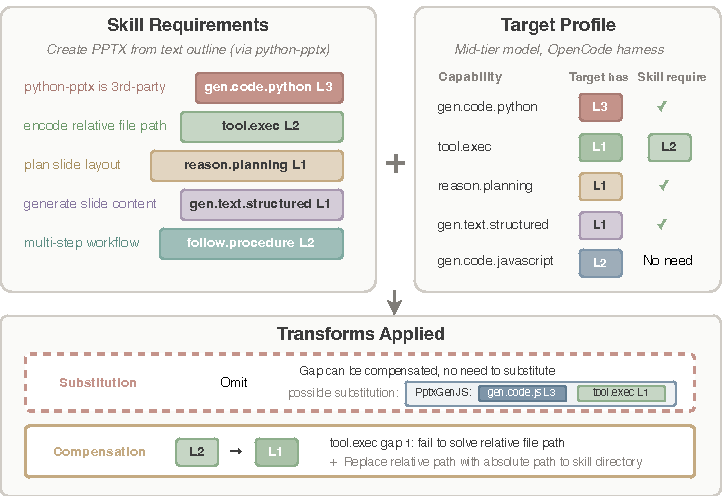
\includegraphics[width=\columnwidth]{figures/compilation-case-study.pdf}
  \caption{对 PPTX 技能进行基于能力的编译。编译器提取技能需求（左），对目标端进行画像（中），并根据缺口应用变换（下）。}
  \label{fig:compilation_case}
\end{figure}

\heading{案例研究。}
图~\ref{fig:compilation_case} 展示了一个真实技能的编译过程；
该技能教代理使用 python-pptx 创建 PPTX 演示文稿。
这个技能要求五项不同等级的原语能力。
目标端与其中四项直接匹配，但 tool.exec 只达到 L1，
而技能需要 L2 才能解析相对文件路径。

编译器识别出一条可能的替代路径：
经由 \emph{gen.code.javascript} 切换到 \emph{PptxGenJS}，即可替换 python-pptx，
并把 tool.exec 的要求降低到 L1。
不过，由于 tool.exec 的缺口只有一个等级，补偿仍是首选。
L2 画像结果显示，该模型在执行命令时无法解析相对文件路径。
于是编译器把绝对路径解析注入编译后的技能中，
用指向技能目录的绝对路径替换相对路径。

\begin{figure*}[t]
  \centering
  \setlength{\abovecaptionskip}{3pt}
  \setlength{\belowcaptionskip}{0pt}
  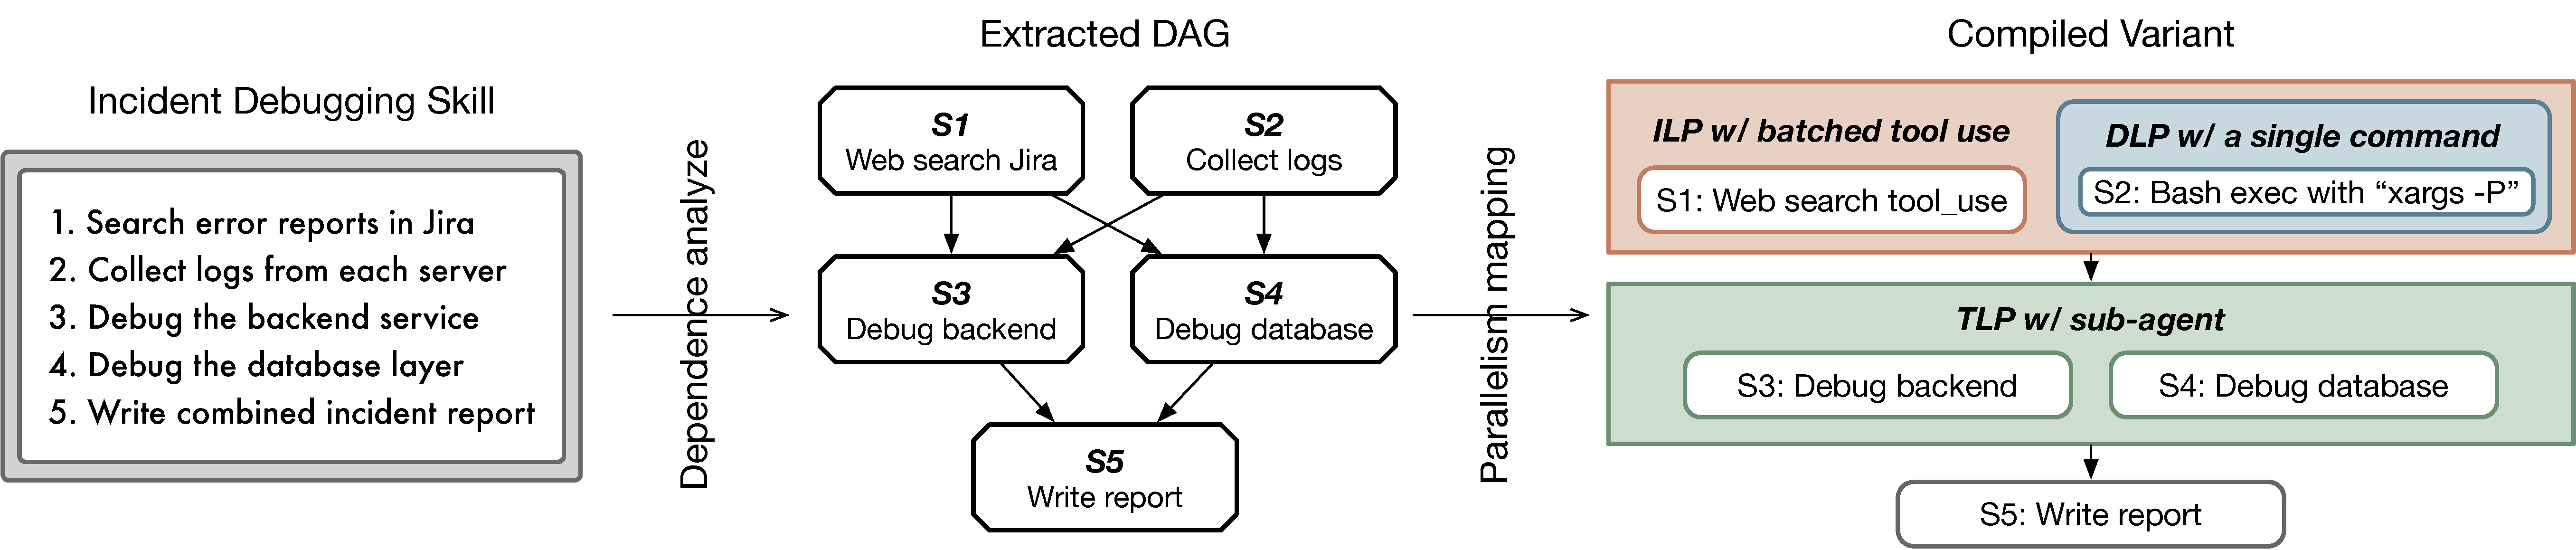
\includegraphics[width=\textwidth]{figures/concurrency_extraction.pdf}
  \caption{在事件响应技能上进行并发性提取。编译器将顺序步骤分解为工作流 DAG，识别步骤之间和步骤内部的并行机会，并把每个机会映射到相应的并发原语。}
  \label{fig:concurrency_extraction}
\end{figure*}

\subsection{环境绑定}
\label{sec:compiler:env}

第二个阶段解决\emph{P3：环境错配}。
编译器不只检查依赖是否已经安装，而是使用内置的\emph{环境绑定技能}，
使技能假设与主机环境相协调，并生成环境绑定脚本。

安装技能时，编译器首先从第一阶段输出的技能与所有显式前置条件中提取依赖清单，
其中包括外部库、CLI 工具和系统服务。
对于清单中的每一项，编译器都会运行轻量级存在性检查（例如 pip show、which）。
已经满足的依赖无需进一步处理。
检查失败时，编译器会执行更深入、感知系统的探测，
以确定如何解决该依赖。
随后，编译器生成幂等的环境绑定脚本；该脚本会在技能执行前检查并修复依赖。
当环境发生变化或环境绑定脚本失败时，
执行会回退到模型，并把脚本输出作为附加上下文传给模型。

\subsection{并发性提取}
\label{sec:compiler:par}

第三个阶段寻找隐藏在显式顺序描述中的并行性。
回顾前文，76\% 的技能包含流程结构（\S\ref{sec:insight:analysis}）。
这些技能用顺序文本描述多步工作流，但并非每一步都真正依赖前一步。

编译器借助 LLM 分析把技能分解为离散步骤，
并识别每一步消费哪些输入、产生哪些输出。
随后，它构建工作流 DAG：节点表示步骤；若步骤 B 消费步骤 A 的输出，
则存在一条从 A 指向 B 的边。
编译器还会分析每个步骤内部可并发执行的子操作。
图~\ref{fig:concurrency_extraction} 用一个事件响应技能展示这一过程。
对于步骤之间或步骤内部的每个并行机会，
编译器都会根据任务结构与代理框架选择并发原语。
\sys 定义了三个并行层级。

\myparagraph{数据级并行（DLP）。}
单个步骤对多个独立数据项应用同一操作，例如对 15 个 CSV 文件分别运行相同分析。
编译器重写该步骤，使用适合技能实现方式的语言级并行原语来并发处理各数据项，
例如 shell 级并行执行、Python 的 multiprocessing，或 JavaScript 的 Promise.all。
DLP 不需要代理框架提供特殊支持。

\myparagraph{指令级并行（ILP）。}
多个彼此独立的步骤各自需要工具调用，并且它们之间没有数据依赖，
例如对一个项目运行八个独立的代码分析脚本。
编译器把相应的 DAG 节点归入同一个并行阶段，并重写技能，
使这些工具调用在一个 LLM 轮次中一并发出，而不是按顺序文本逐个发出。
编译器还会在技能中标注：批处理完成后，应将哪些步骤输出绑定回哪些下游 DAG 输入。
ILP 要求代理框架支持批量工具分派。

\myparagraph{线程级并行（TLP）。}
工作流可以分解为需要多轮推理的独立子任务，
例如调试三个彼此独立的服务。
编译器重写技能，把每个子任务提取为单独的子代理块；
每个块都带有明确的任务描述、声明的输入上下文，以及可由父工作流消费的预期输出。
标注会将该块标记为交由子代理分派，
运行时因此在各自会话中为每个块生成一个子代理，并把返回的输出合并回 DAG。
TLP 要求代理框架支持生成子代理。

若目标代理框架不具备某个机会所需的原语，该机会就回退为顺序执行。
对于每个可行机会，编译器要么重写技能指令，让数据项并发执行（DLP），
要么生成执行标注，使并行结构显式化：ILP 使用跨 DAG 节点的并行阶段，
TLP 使用带输入、输出契约的子代理任务块。
运行时读取这些标注，并通过对应的代理框架原语进行分派。
